\section{Digital Sound}

\frame{\tableofcontents[currentsection]}

\begin{frame}
  \frametitle{Sound Representation}
  \begin{itemize}
    \item How does sound/music get represent in software?
    \item Two fundamentally different approaches
  \end{itemize}
\end{frame}


\subsection{Midi Files}

\frame{\tableofcontents[currentsubsection]}


\begin{frame}
  \frametitle{Storing Music: The Midi Way}
  \begin{itemize}
    \item For each note, store
          \begin{itemize}
            \item Note
            \item Duration
            \item Loudness
            \item Timbre
          \end{itemize}
    \item Similar to storing sheet music
  \end{itemize}
  \vskip5mm
  \structure{Example}
  \begin{center}
    \begin{tabular}{rccccccccc}
      \textbf{Note} & E5 & D$\sharp$5 & E5 & D$\sharp$5 & E5 & B4 & D5 & C5 & A4 \\
      \textbf{Duration} & $\nicefrac12$ & $\nicefrac12$ & $\nicefrac12$ & $\nicefrac12$ & $\nicefrac12$ & $\nicefrac12$ & $\nicefrac12$ & $\nicefrac12$ & $1$ \\
      \textbf{Loudness} & \multicolumn{9}{c}{pianissimo} \\
      \textbf{Timbre} & \multicolumn{9}{c}{piano} \\
    \end{tabular}
  \end{center}
\end{frame}

\begin{frame}
  \frametitle{Midi Files}
  \structure{Advantages}
  \begin{itemize}
    \item Very compact
    \item Easy to use for music composition
  \end{itemize}
  \vskip5mm
  \structure{Disadvantages}
  \begin{itemize}
    \item Can only store music, not sound
          \begin{itemize}
            \item I.e.~cannot store voice
          \end{itemize}
    \item Sounds very mechanical (plays too perfectly)
    \item Cannot represent ``feeling'' (i.e.~conscious ``mistakes'' in music performance)
  \end{itemize}
\end{frame}


\subsection{Wave Files}

\frame{\tableofcontents[currentsubsection]}

\begin{frame}
  \frametitle{Wave Files}
  \begin{itemize}
    \item Encode the sound wave itself
    \item How to write an arbitrary sound wave to file?
          \begin{itemize}
            \item Sound wave can be infinitely detailed
            \item We only have finite storage available
          \end{itemize}
  \end{itemize}
  \begin{center}
    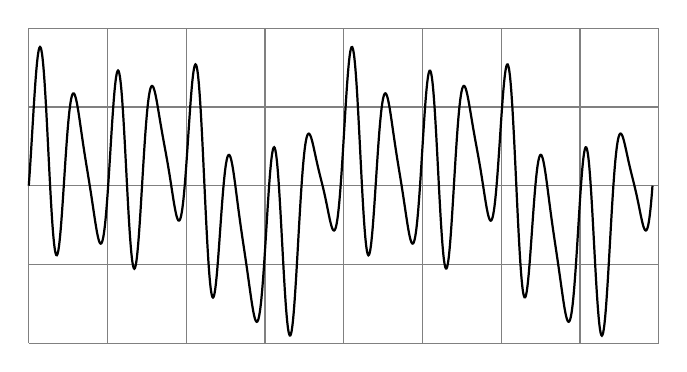
\begin{tikzpicture}
      \draw[thin,gray] (0,-2) grid (8,2);
      \draw[thick] plot[domain=0:720,x=0.011cm,y=1cm,samples=1000,smooth] (\x,{sin(8*\x)+0.75 * sin(7*\x)*sin(5*\x)+0.5*sin(\x)});
    \end{tikzpicture}
  \end{center}
\end{frame}

\begin{frame}
  \frametitle{Sampling}
  \begin{itemize}
    \item Say wave is described by mathematical function $f$
    \item We compute $f$ at $N$ points (uniformly distributed)
          \begin{itemize}
            \item E.g.~every 0.1 seconds: $f(0), f(0.1), f(0.2), f(0.3), \dots$
            \end{itemize}
    \item We store only those values
  \end{itemize}
  \begin{center}
    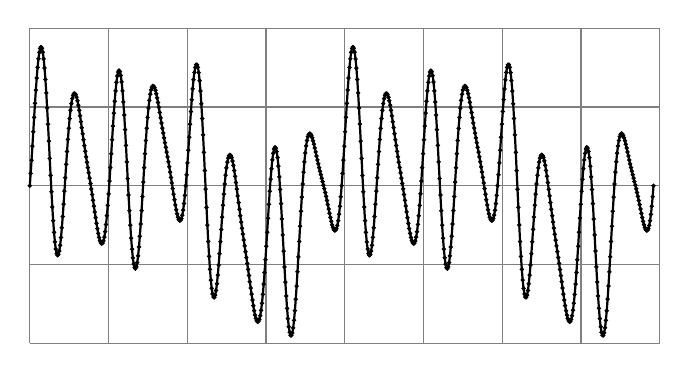
\begin{tikzpicture}
      \draw[thin,gray] (0,-2) grid (8,2);
      \visible<1-2>{
        \draw[thick] plot[domain=0:720,x=0.011cm,y=1cm,samples=1000,smooth] (\x,{sin(8*\x)+0.75 * sin(7*\x)*sin(5*\x)+0.5*sin(\x)});
      }
      \visible<2-3>{
        \foreach[evaluate={sin(8*\x)+0.75 * sin(7*\x)*sin(5*\x)+0.5*sin(\x)} as \y] \x in {0,...,720} {
          \draw[fill] (\x*0.011,\y) circle [radius=0.02cm];
        }
      }
    \end{tikzpicture}
  \end{center}
\end{frame}

\begin{frame}
  \frametitle{Sampling Rate}
  \begin{itemize}
    \item How many samples to take?
          \begin{itemize}
            \item Many samples: precise, but much storage space
            \item Few samples: little storage, but bad quality
          \end{itemize}
  \end{itemize}
  \begin{center}
    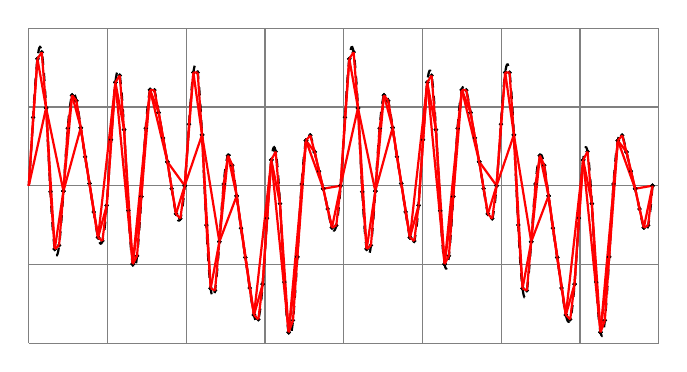
\begin{tikzpicture}
      \draw[thin,gray] (0,-2) grid (8,2);
      \draw[thick,dashed] plot[domain=0:720,x=0.011cm,y=1cm,samples=1000,smooth] (\x,{sin(8*\x)+0.75 * sin(7*\x)*sin(5*\x)+0.5*sin(\x)});

      \visible<1>{
        \foreach[evaluate={sin(8*\x)+0.75 * sin(7*\x)*sin(5*\x)+0.5*sin(\x)} as \y,
                 remember=\y as \lasty (initially 0),
                 remember=\x as \lastx (initially 0)] \x in {20,40,...,720} {
          \draw[fill] (\x*0.011,\y) circle [radius=0.02cm];
          \draw[red,thick] (\lastx*0.011,\lasty) -- (\x*0.011,\y);
        }
      }

      \visible<2>{
        \foreach[evaluate={sin(8*\x)+0.75 * sin(7*\x)*sin(5*\x)+0.5*sin(\x)} as \y,
                 remember=\y as \lasty (initially 0),
                 remember=\x as \lastx (initially 0)] \x in {10,20,...,720} {
          \draw[fill] (\x*0.011,\y) circle [radius=0.02cm];
          \draw[red,thick] (\lastx*0.011,\lasty) -- (\x*0.011,\y);
        }
      }

      \visible<3>{
        \foreach[evaluate={sin(8*\x)+0.75 * sin(7*\x)*sin(5*\x)+0.5*sin(\x)} as \y,
                 remember=\y as \lasty (initially 0),
                 remember=\x as \lastx (initially 0)] \x in {5,10,...,720} {
          \draw[fill] (\x*0.011,\y) circle [radius=0.02cm];
          \draw[red,thick] (\lastx*0.011,\lasty) -- (\x*0.011,\y);
        }
      }
    \end{tikzpicture}
  \end{center}
  \vskip-5mm
  \begin{overprint}
    \onslide<1>
    \begin{center}
      36 samples
    \end{center}
    \onslide<1>
    \begin{center}
      72 samples
    \end{center}
    \onslide<1>
    \begin{center}
      144 samples
    \end{center}
  \end{overprint}
\end{frame}

\begin{frame}
  \frametitle{Nyquist Frequency}
  \begin{itemize}
    \item Human ear hears frequencies \SI{20}{\hertz} till \SI{20000}{\hertz}
    \item \link{https://en.wikipedia.org/wiki/Nyquist\%E2\%80\%93Shannon_sampling_theorem}{Nyquist} said you need to sample at twice
          the maximum frequency
    \item I.e.~we should take \SI{40000}{} samples per second
    \item In practice \SI{44100}{\hertz} is often used
  \end{itemize}
\end{frame}

\begin{frame}
  \frametitle{Vertical Subdivisions}
  \begin{itemize}
    \item Sampling rate determines horizontal subdivisions
    \item What about vertical subdivisions?
  \end{itemize}
  \begin{center}
    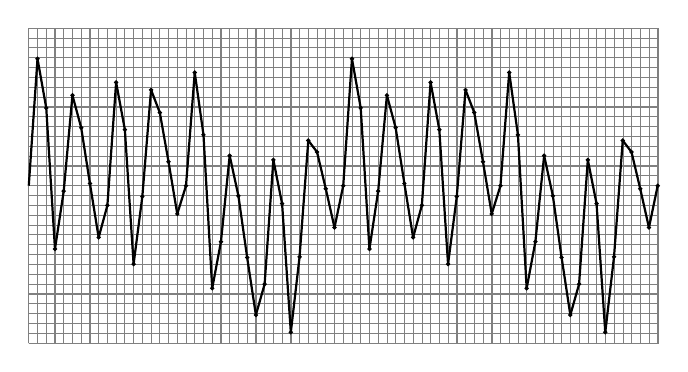
\begin{tikzpicture}
      \visible<1>{
        \draw[thin,gray] (0,-2) grid[xstep=0.111cm,ystep=1cm] (8,2);
      }
      \visible<2>{
        \draw[thin,gray] (0,-2) grid[xstep=0.111cm,ystep=0.5cm] (8,2);
      }
      \visible<3>{
        \draw[thin,gray] (0,-2) grid[xstep=0.111cm,ystep=0.25cm] (8,2);
      }
      \visible<4>{
        \draw[thin,gray] (0,-2) grid[xstep=0.111cm,ystep=0.125cm] (8,2);
      }
      \foreach[evaluate={sin(8*\x)+0.75 * sin(7*\x)*sin(5*\x)+0.5*sin(\x)} as \y,
               remember=\y as \lasty (initially 0),
               remember=\x as \lastx (initially 0)] \x in {10,20,...,720} {
        \draw[fill] (\x*0.0111,\y) circle [radius=0.02cm];
        \draw[thick] (\lastx*0.0111,\lasty) -- (\x*0.0111,\y);
      }
    \end{tikzpicture}
  \end{center}
\end{frame}

\begin{frame}
  \frametitle{Vertical Subdivisions}
  \begin{itemize}
    \item Amount of vertical subdivisions determines precision
    \item Say 2 bit per sample
    \item Allows for only 4 amplitudes
    \item Each sample has to be ``rounded'' to the nearest amplitude
  \end{itemize}
  \begin{overprint}
    \onslide<1-2>
    \begin{center}
      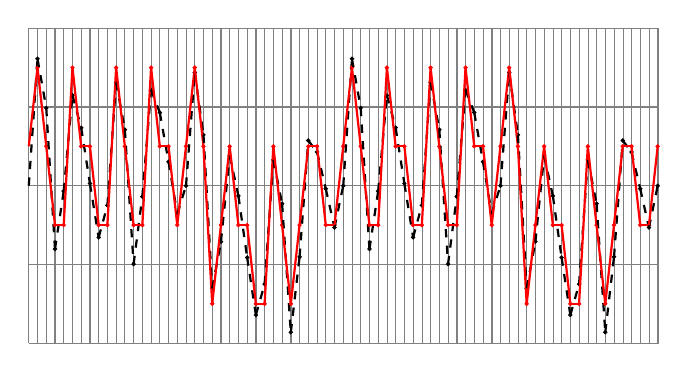
\begin{tikzpicture}
        \draw[thin,gray] (0,-2) grid[xstep=0.111cm,ystep=1cm] (8,2);

        \foreach[evaluate={sin(8*\x)+0.75 * sin(7*\x)*sin(5*\x)+0.5*sin(\x)} as \exacty,
                 evaluate={round(\exacty+0.5)-0.5} as \y,
                 remember=\y as \lasty (initially 0.5),
                 remember=\x as \lastx (initially 0),
                 remember=\exacty as \lastexacty (initially 0)] \x in {10,20,...,720} {

          \visible<1>{
            \draw[fill] (\x*0.0111,\exacty) circle [radius=0.02cm];
            \draw[thick,dashed] (\lastx*0.0111,\lastexacty) -- (\x*0.0111,\exacty);
          }
          \draw[fill,red] (\x*0.0111,\y) circle [radius=0.02cm];
          \draw[thick,red] (\lastx*0.0111,\lasty) -- (\x*0.0111,\y);
        }
      \end{tikzpicture}
    \end{center}
    \onslide<3>
    \begin{center}
      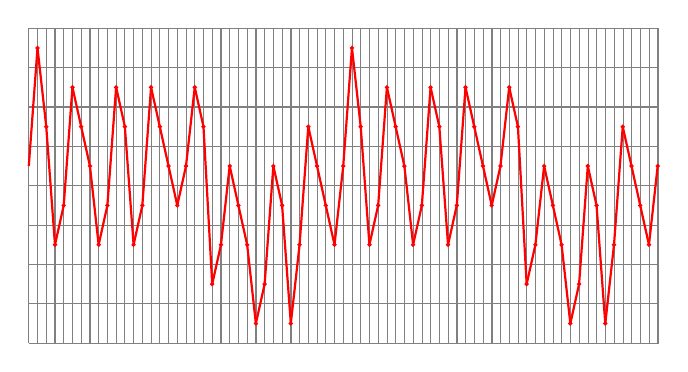
\begin{tikzpicture}
        \draw[thin,gray] (0,-2) grid[xstep=0.111cm,ystep=0.5cm] (8,2);

        \foreach[evaluate={sin(8*\x)+0.75 * sin(7*\x)*sin(5*\x)+0.5*sin(\x)} as \exacty,
                 evaluate={round((\exacty+0.25)*2)/2-0.25} as \y,
                 remember=\y as \lasty (initially 0.25),
                 remember=\x as \lastx (initially 0),
                 remember=\exacty as \lastexacty (initially 0)] \x in {10,20,...,720} {

          \draw[fill,red] (\x*0.0111,\y) circle [radius=0.02cm];
          \draw[thick,red] (\lastx*0.0111,\lasty) -- (\x*0.0111,\y);
        }
      \end{tikzpicture}
    \end{center}
    \onslide<4>
    \begin{center}
      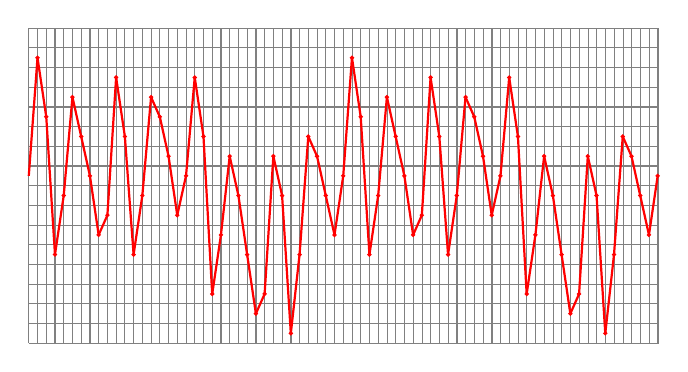
\begin{tikzpicture}
        \draw[thin,gray] (0,-2) grid[xstep=0.111cm,ystep=0.25cm] (8,2);

        \foreach[evaluate={sin(8*\x)+0.75 * sin(7*\x)*sin(5*\x)+0.5*sin(\x)} as \exacty,
                 evaluate={round((\exacty+0.125)*4)/4-0.125} as \y,
                 remember=\y as \lasty (initially 0.125),
                 remember=\x as \lastx (initially 0),
                 remember=\exacty as \lastexacty (initially 0)] \x in {10,20,...,720} {

          \draw[fill,red] (\x*0.0111,\y) circle [radius=0.02cm];
          \draw[thick,red] (\lastx*0.0111,\lasty) -- (\x*0.0111,\y);
        }
      \end{tikzpicture}
    \end{center}
    \onslide<5>
    \begin{center}
      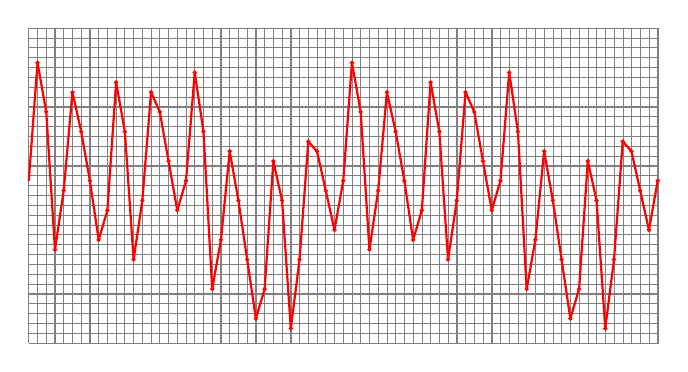
\begin{tikzpicture}
        \draw[thin,gray] (0,-2) grid[xstep=0.111cm,ystep=0.125cm] (8,2);

        \foreach[evaluate={sin(8*\x)+0.75 * sin(7*\x)*sin(5*\x)+0.5*sin(\x)} as \exacty,
                 evaluate={round((\exacty+0.0625)*8)/8-0.0625} as \y,
                 remember=\y as \lasty (initially 0.0625),
                 remember=\x as \lastx (initially 0),
                 remember=\exacty as \lastexacty (initially 0)] \x in {10,20,...,720} {

          \draw[fill,red] (\x*0.0111,\y) circle [radius=0.02cm];
          \draw[thick,red] (\lastx*0.0111,\lasty) -- (\x*0.0111,\y);
        }
      \end{tikzpicture}
    \end{center}
  \end{overprint}
  \begin{overprint}
    \onslide<1-2>
    \begin{center}
      2 bits per sample
    \end{center}
    \onslide<3>
    \begin{center}
      4 bits per sample
    \end{center}
    \onslide<4>
    \begin{center}
      5 bits per sample
    \end{center}
    \onslide<5>
    \begin{center}
      6 bits per sample
    \end{center}
  \end{overprint}
\end{frame}

\begin{frame}
  \frametitle{Bit Depth}
  \begin{itemize}
    \item Let's say 8 bits
    \item Means 256 vertical subdivisions
    \item Question: which interval is being subdivided? $[-1,1]$?
    \item Sound can be as loud as it wants
    \item Original wave function $f(x)$ can take \emph{any} value
    \item So, are we to divide $[-\infty,\infty]$ in 256 subintervals?
  \end{itemize}
\end{frame}

\begin{frame}
  \frametitle{Bit Depth}
  \begin{itemize}
    \item We pick an arbitrary interval, say $[-1, 1]$
    \item We say the wave function has to fit inside this interval
    \item $f(t) = 1$ or $f(t) = -1$ corresponds to ``loudest''
    \item How loud it actually is depends on listener's volume control 
  \end{itemize}
  \begin{center}
    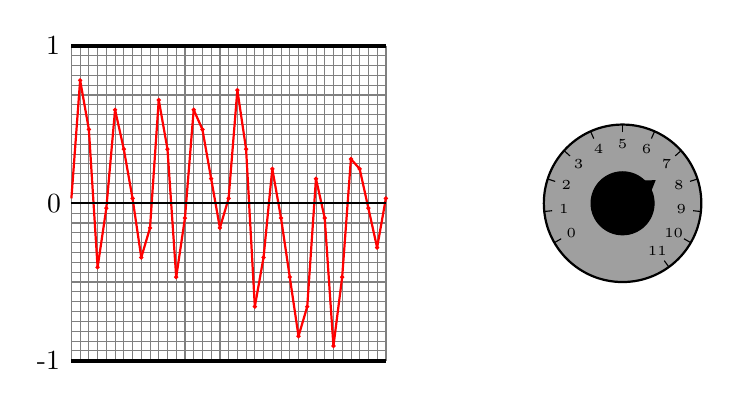
\begin{tikzpicture}
        \draw[thin,gray] (0,-2) grid[xstep=0.111cm,ystep=0.125cm] (4,2);

        \foreach[evaluate={sin(8*\x)+0.75 * sin(7*\x)*sin(5*\x)+0.5*sin(\x)} as \exacty,
                 evaluate={round((\exacty+0.0625)*8)/8-0.0625} as \y,
                 remember=\y as \lasty (initially 0.0625),
                 remember=\x as \lastx (initially 0),
                 remember=\exacty as \lastexacty (initially 0)] \x in {10,20,...,360} {

          \draw[fill,red] (\x*0.0111,\y) circle [radius=0.02cm];
          \draw[thick,red] (\lastx*0.0111,\lasty) -- (\x*0.0111,\y);
        }
       
        \draw[ultra thick] (0,2) -- (4,2) node[at start,anchor=east] {1};
        \draw[thick] (0,0) -- (4,0) node[at start,anchor=east] {0};
        \draw[ultra thick] (0,-2) -- (4,-2) node[at start,anchor=east] {-1};

        \begin{scope}[xshift=7cm]
          \draw[thick,fill=gray!75!white] (0,0) circle [radius=1cm];
          \draw[fill=black] (0,0) circle [radius=4mm];
          \draw[fill=black] (25:0.4) -- (35:0.5) -- (45:0.4) -- cycle;
          
          \foreach[count=\i from 0,evaluate={-\x+90} as \a] \x in {-120,-96,...,144} {
            \draw (\a:0.9) -- (\a:1);
            \node[font=\tiny] at (\a:0.75) {\i};
          }
        \end{scope}
    \end{tikzpicture}
  \end{center}
\end{frame} % https://www.youtube.com/watch?v=DzLP2Z7JVZA

\begin{frame}
  \frametitle{Audio Formats}
  \structure{Audio CD}
  \begin{itemize}
    \item Audio CD contains raw wave data
    \item For example, Audio CD is 16 bit, \SI{44.1}{\kilo\hertz}, stereo
          \[
            2 \cdot 16 \cdot \num{44100} = \num{1411200} \textrm{bit/s}
          \]
    \item Audio capacity: 74 to 80 minutes, or \SI{750}{\mega\byte} to \SI{810}{\mega\byte}
  \end{itemize}
  \vskip5mm
  \structure{MP3, M4A, \dots}
  \begin{itemize}
    \item Audio formats such as MP3 are compressed wave files
    \item MP3 is $7-11\times$ smaller than wave files
  \end{itemize}
\end{frame}




%%% Local Variables:
%%% mode: latex
%%% TeX-master: "sound"
%%% End:
